% !TeX encoding = UTF-8
% !TeX spellcheck = en_US
% !TeX root = collegeProject.tex

\documentclass[a4paper, 14pt, openany]{report}

% For manipulating title alignments.
\usepackage{titlesec}
% For including pictures
\usepackage{graphicx}
% To disable numbering
\usepackage{sectsty}
% Times New Roman Like Font
\usepackage{mathptmx}
% For increasing font sizes
\usepackage{extsizes}
% Margin of the report document
\usepackage[left=1.5in,right=1in,top=1.5in,bottom=1in]{geometry}
% For two column layout
\usepackage{multicol}
% Lorem Ipsum 
\usepackage{lipsum}
% Gantt Chart 
\usepackage{pgfgantt}
% for list of abbreviations
\usepackage{enumitem}
% For date and time
\usepackage{datetime}

% Line Spacing
\linespread{1.5}

% Title spacing
\chapternumberfont{\fontsize{18pt}{18pt}\selectfont\center}
\chaptertitlefont{\fontsize{18pt}{18pt}\selectfont\center}

\sectionfont{\fontsize{16}{16}\selectfont}
\subsectionfont{\fontsize{15}{15}\selectfont}

\usepackage{caption}

\title{Gandaki College of Engineering and Science Academic Project Report Template}
\author{Arjun Prasad Adhikari}
\date{2020 April 19}

\graphicspath{{figures/}}

\begin{document}
	
	\pagenumbering{gobble}
	
	\maketitle

	\begin{titlepage}
		\begin{center}
			A Minor Project Proposal on \\
			\textbf{TITLE OF PROJECT}
			\vskip1cm
			Submitted in partial fulfillment of the requirements for the degree of \\ 
             Bachelor of Engineering in Software Engineering at Pokhara University
			
			\vskip1.5cm
			
			\textbf{\textit{By\\}}
			\textbf{TEAM MEMBER 1 \\ TEAM MEMBER 2 \\ TEAM MEMBER 3}
			
			\vskip2cm
			
			
\includegraphics[width=4cm]{logo/gces.png}
			
			\vskip2cm
			
			\textbf{Department of Research and Development \\ GANDAKI COLLEGE OF ENGINEERING AND SCIENCE}
			
			Lamachaur, Kaski, Nepal
			\vskip1cm
			 (Month, Year)
			
			\newpage
			\pagenumbering{gobble}
			
			A Minor Project Proposal on \\
			\textbf{TITLE OF PROJECT}
			\vskip1cm
			Submitted in partial fulfillment of the requirements for the degree of \\ 
Bachelor of Engineering in Software Engineering at Pokhara University
			
			
			\vskip1.5cm
			
			\textbf{\textit{By\\}}
			\textbf{TEAM MEMBER 1 \\ TEAM MEMBER 2 \\ TEAM MEMBER 3}
			
			\vskip1cm
			
			\textbf{\textit{Supervisor}}
			\textbf{\\ YOUR SUPERVISOR NAME}			
			
			\vskip1cm
			
			
\includegraphics[width=4cm]{logo/gces.png}
			
			\vskip1cm
			
			\textbf{Department of Research and Development \\ GANDAKI COLLEGE OF ENGINEERING AND SCIENCE}
			
			Lamachaur, Kaski, Nepal
			
			\vskip1cm
			 (Month, Year)

		\end{center}
	\end{titlepage}
	
	\pagenumbering{roman}

	
\section*{\center APPROVAL CERTIFICATE}

		This project entitled "YOUR PROJECT NAME" prepared and submitted by "PROJECT PARTNERS" under the supervision of "YOUR SUPERVISOR NAME" in partial fulfillment of the requirements for the Degree of Bachelor of Engineering in Software Engineering has been examined and is recommended for approval and acceptance.\\
\linebreak
\textbf{Date of Evaluation:} September 12th, 2014\\
\linebreak

% Multi column view
\begin{multicols}{2}
	
	\noindent\rule{6cm}{0.1pt}\\
	\textbf{Supervisor's name} \\
	(Project Supervisor)\\
	\linebreak
	
		\noindent\rule{6cm}{0.1pt}\\
	\textbf{Er. Sujan Tamrakar} \\
	(Project Head) \\
	\textbf{Research and Development ,} \\
	\textbf{Gandaki College of Engineering\\ and Science}
	
	\columnbreak
	
	\noindent\rule{6cm}{0.1pt}\\
	\textbf{Falano Dhimkana} \\
	(External Examiner) \\ 
	\linebreak
	 
	\noindent\rule{6cm}{0.1pt}\\
	\textbf{Mr. Ashok Raj Parajuli} \\
	(Vice Principal) \\
	\textbf{Gandaki College of Engineering\\  and Science}\\
	
	
	
	                   
\end{multicols} 
% End multi column view
	
	
	




	
\section*{\center ACKNOWLEDGEMENT}
	
We would like to express our heart full thanks to our project supervisor \textbf{YOUR SUPERVISOR NAME}, who supported us to do this project by giving valuable suggestions and guidelines during the development phase. We are thankful to the principal \textbf{Mr. Birendra Khadka} and the vice-principal \textbf{Mr. Ashok Raj Parajuli} for supporting us during the entire project. We are also thankful to all our teachers and staffs for their assistance, support and encouragement to complete our project. A special gratitude to \textbf{Mr. Sujan Tamrakar}, HOD, Department of Research and Development for the guidance and investigation.\\
\linebreak
Finally, we would like to thank all our friends and library staffs who helped us by providing several suggestions and comments to make this project successful.\\
\linebreak
YOUR NAME 1\\
YOUR NAME 2\\
YOUR NAME 3\\
\linebreak
Gandaki College of Engineering and Science\\
Lamachaur, Pokhara, Kaski
	\section*{\center ABSTRACT}


Pahichaan is a web application which allows the user to connect with each
other. It provides a user-friendly platform for users to post their recognition status. Users are allowed to post the pictures of their honors, awards, certificates and text status. Not limited to this, they can connect to each other and react on connection’s post and perform texting to connections. Similarly, connections will get notified of each other’s activity.
	
	\tableofcontents
	\listoffigures
	\listoftables
	
	\newlist{abbrv}{itemize}{1}
\setlist[abbrv,1]{label=,labelwidth=1in,align=parleft,itemsep=0.1\baselineskip,leftmargin=!}

\chapter*{List of Abbreviations}

\begin{abbrv}
	
	\item[AHSS]			Advanced High Strength Steel
	\item[HTML]			Hyper Text Transfer Protocol
	
\end{abbrv}
	
	
	\begin{center}
	\chapter{INTRODUCTION}
\end{center}

\pagenumbering{arabic}
	
\section{BACKGROUND}
\par
\lipsum[1]

\section{PROBLEM STATEMENT}
\par
\lipsum[2]

\section{OBJECTIVES}
\par
\lipsum[3]

\section{IMPLICATIONS}
\par
\lipsum[4]		
	\begin{center}
	\chapter{LITERATURE REVIEW}
\end{center}

\par
\lipsum[4]
\vspace{1cm}

\begin{table}[h!]
  \begin{center}
    \label{tab:table1}
    \begin{tabular}{|l|l|l|l|l|} 
    \hline
      & Project 1 & Project 2 & Project 3 & Our Project \\
      \hline
Feature 1 & Yes       & Yes       & No        & No        \\
Feature 2 & Yes       & No        & Yes       & No        \\
Feature 3 & No        & No        & No        & Yes       \\
Feature 4 & No        & Yes       & No        & No        \\
Feature 5 & Yes       & No        & Yes       & No        \\
	\hline
    \end{tabular}
    \caption{Literature Review}
  \end{center}
\end{table}

\lipsum[4]
	\begin{center}
	\chapter{TOOLS AND METHODOLOGIES}
\end{center}
	
\section{REQUIRED TOOLS}

	\par
	For the development of our project, we will be using the following tools.
	\linebreak
	

\begin{table}[h!]
  \begin{center}
    \label{tab:table1}	

	\begin{tabular}{|c|c|}
        \hline
        Tool & Description \\
        \hline
        Python &  Backend Processing \\
        Django &  Backend Framework\\
        ... &  ...\\
        \hline
    \end{tabular}
    \\[3em] % Gap between table and caption
    \caption{Tools required for "Project Name"}
  \end{center}
\end{table}

\section{APPROACH USED}
\lipsum[4]
\begin{figure}[h!]
	\begin{center}
		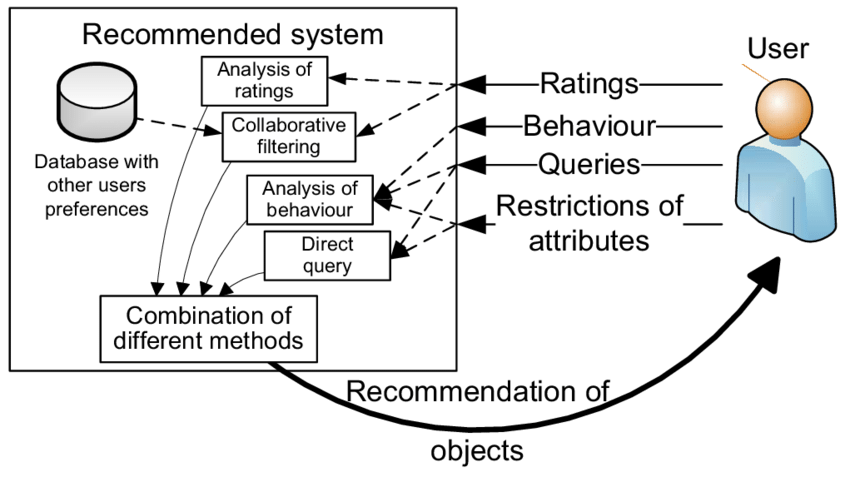
\includegraphics[width=1\textwidth]{algo/algo1.png}
	\end{center}
	\caption{How Recommendation of objects is done ?}
\end{figure}
\linebreak
\lipsum[4]


\subsection{USE CASE DIAGRAM}
\lipsum[4]
\begin{figure}[h!]
	\begin{center}
		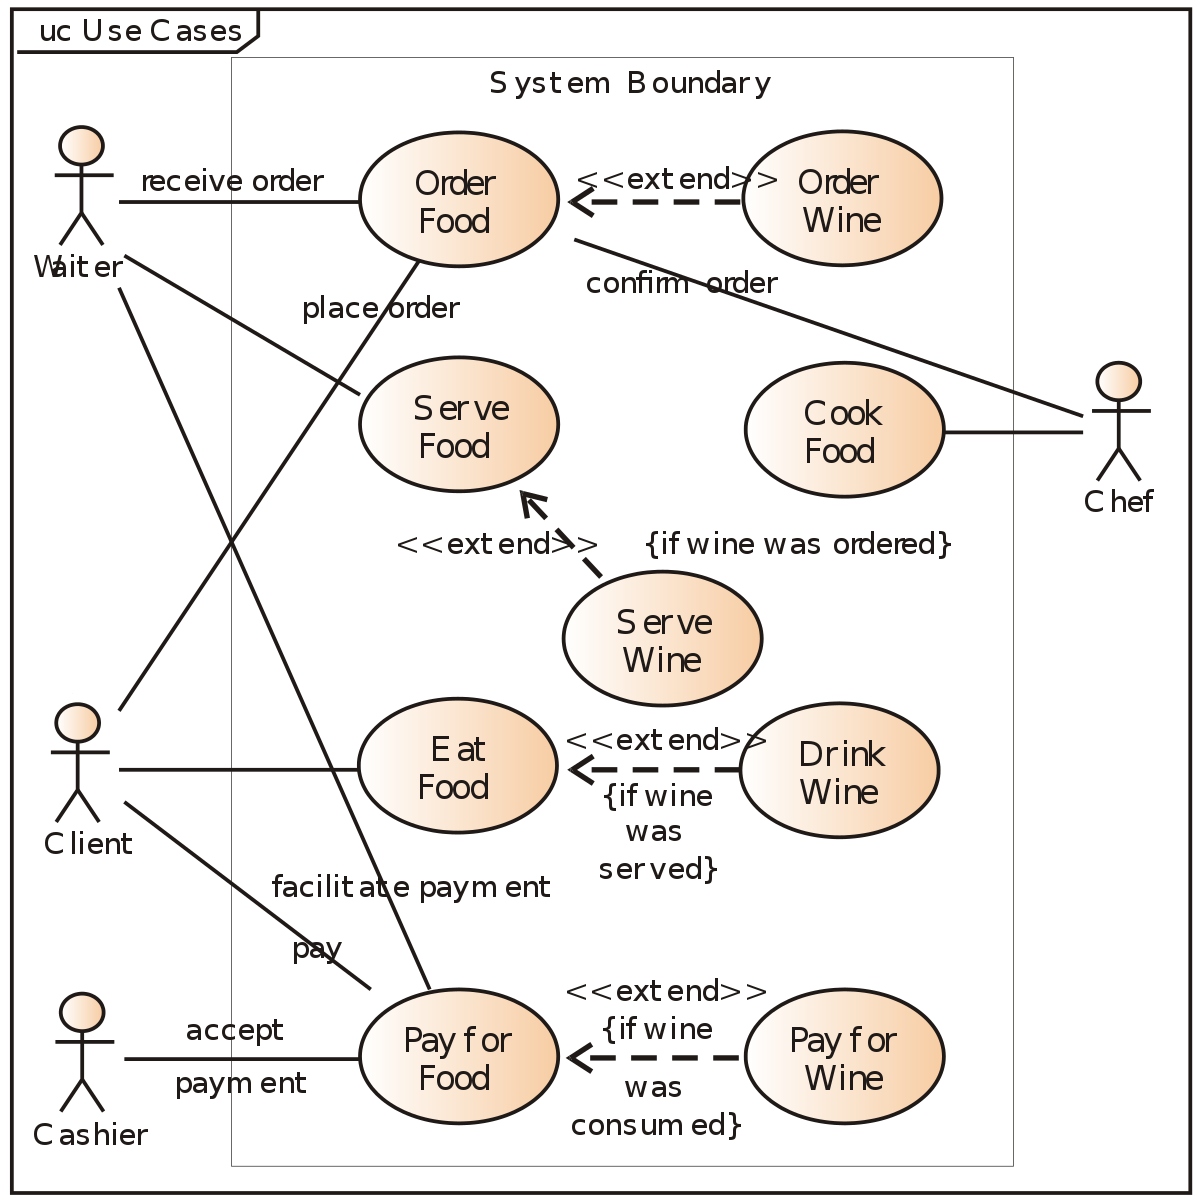
\includegraphics[width=1\textwidth]{uml/usecase.png}
	\end{center}
	\caption{Use case Diagram}
\end{figure}

\subsection{ENTITY RELATIONSHIP DIAGRAM}
\lipsum[4]
\begin{figure}[h!]
	\begin{center}
		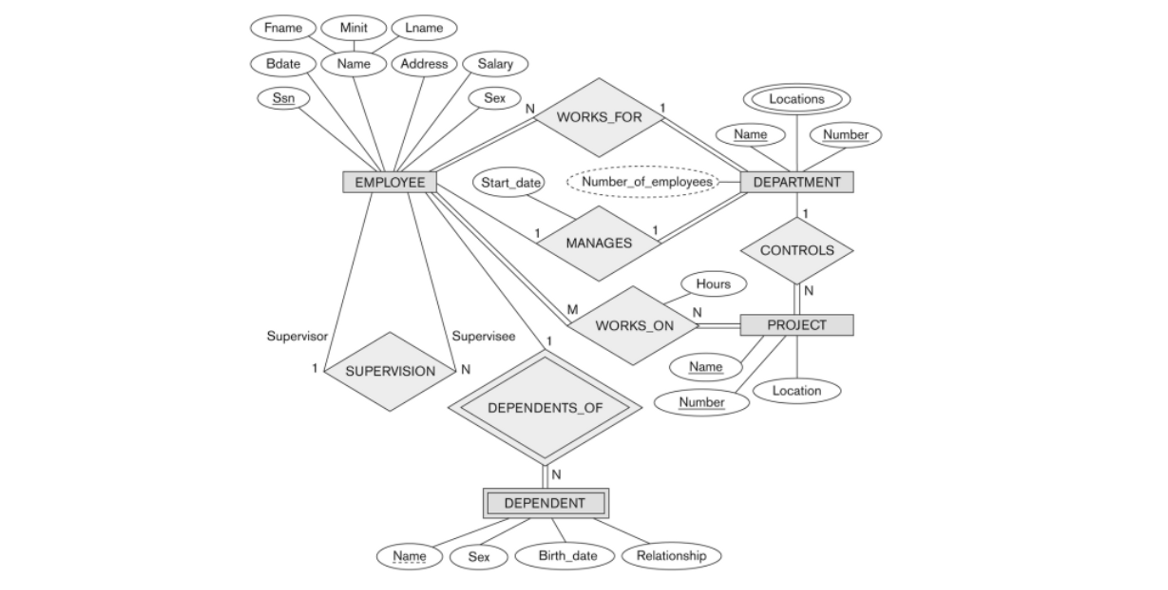
\includegraphics[width=1.3\textwidth]{uml/er.png}
	\end{center}
	\caption{Entity Relationship Diagram}
\end{figure}

\subsection{SYSTEM SEQUENCE DIAGRAM}
\lipsum[4]
\begin{figure}[h!]
	\begin{center}
		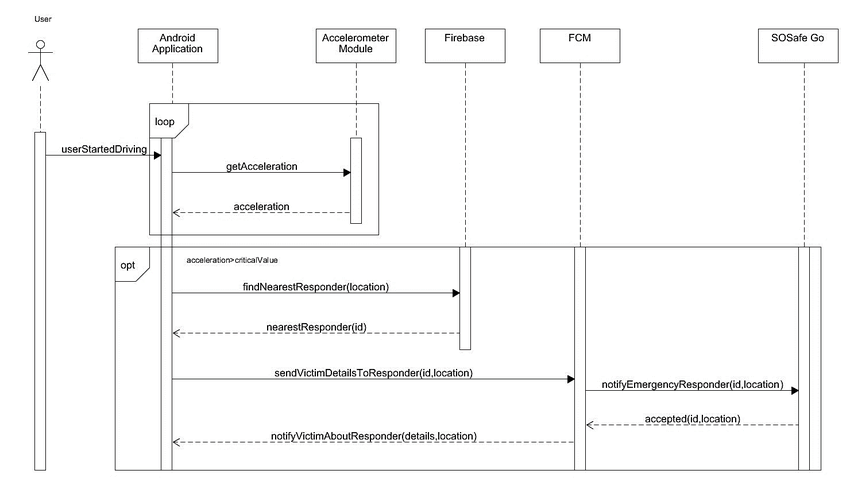
\includegraphics[width=1\textwidth]{uml/ssd.png}
	\end{center}
	\caption{System Sequence Diagram}
\end{figure}

\subsection{CLASS DIAGRAM}
\lipsum[4]
\begin{figure}[h!]
	\begin{center}
		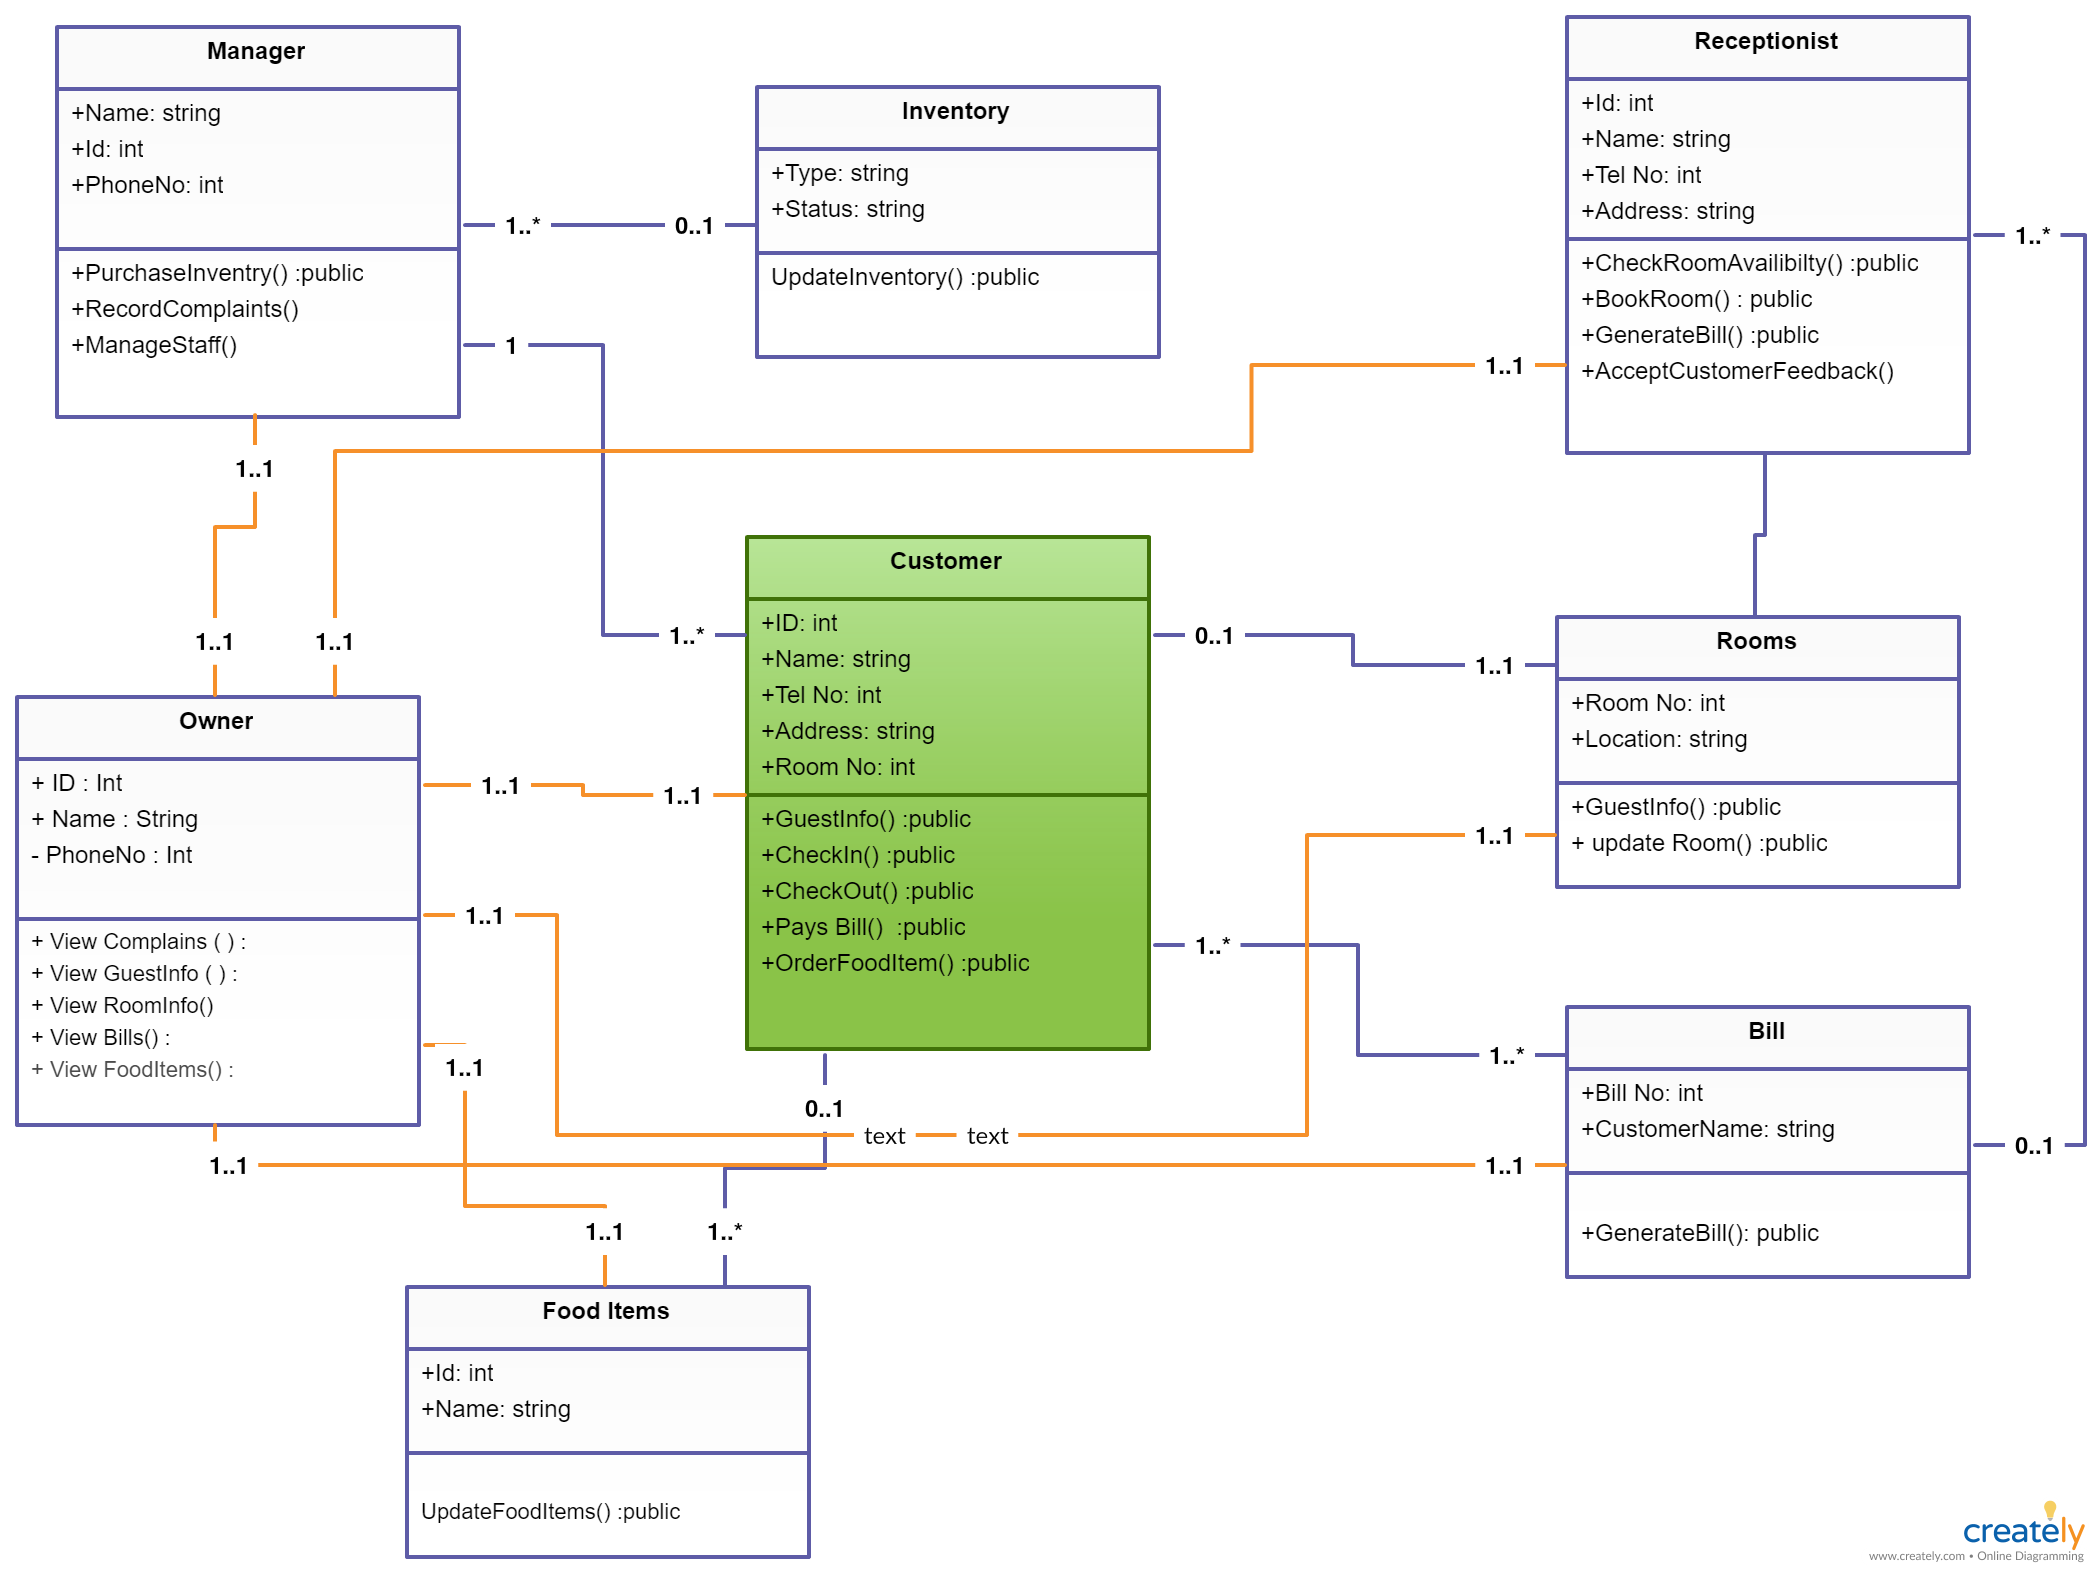
\includegraphics[width=1\textwidth]{uml/class.png}
	\end{center}
	\caption{Class Diagram}
\end{figure}
	\begin{center}
	\chapter{TESTING}
\end{center}
\section{OBJECTIVES OF TESTING}
The objectives of testing are :
\begin{enumerate}
	\item One
	\item Two
	\item Three
\end{enumerate}

\section{TEST CASES}
Following test cases were analysed :
\begin{enumerate}
	\item One
	\item Two
	\item Three
\end{enumerate}

\section{TESTING GOALS}
	\begin{center}
	\chapter{TIMELINE CHART}
\end{center}
\par
\begin{figure}
	\centering
	\begin{ganttchart}[
		inline, 
		bar inline label anchor=west,
		bar inline label node/.append style={anchor=west, text=white},
		bar/.append style={fill=gray!120!black,}, 
		bar height=1,]{0}{18}
		\gantttitlelist{0, ..., 18}{1}\\
		\ganttbar[inline=false]{Design}{0}{3}
		\ganttbar{J1}{0}{3}
		\ganttbar{J2}{3}{4}
		\ganttbar{}{5}{18}\\
		\ganttbar[inline=false]{M2}{0}{5}
		\ganttbar{J2}{5}{8}
		\ganttbar{J1}{8}{12}
		\ganttbar{}{12}{18}
	\end{ganttchart}
	\caption{To demonstrate Flow shop Scheduling}
\end{figure}

	\begin{center}
	\chapter{RESULTS AND DISCUSSION}
\end{center}
\section{FUTURE RESEARCH AND RECOMMENDATIONS}
	\begin{center}
	\chapter{SNAPSHOTS}
\end{center}
\section{WIRE FRAMES}

\begin{figure}[h!]
	\begin{center}
		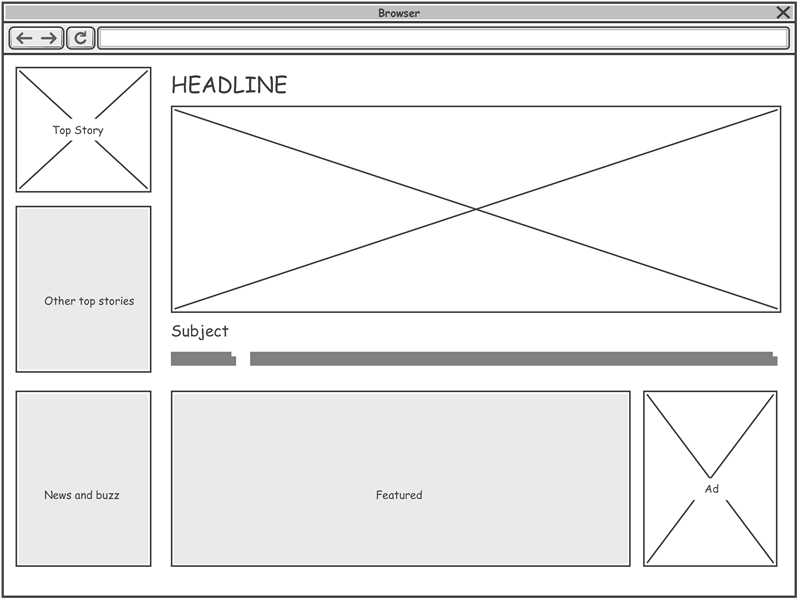
\includegraphics[width=1\textwidth]{wireframes/wireframe1.png}
	\end{center}
	\caption{Wireframe 1}
\end{figure}

\begin{figure}[h!]
	\begin{center}
		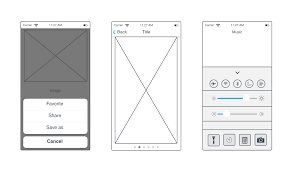
\includegraphics[width=1\textwidth]{wireframes/wireframe2.png}
	\end{center}
	\caption{Wireframe 2}
\end{figure}

\newpage
\section{USER INTERFACES}

\begin{figure}[h!]
	\begin{center}
  		
\includegraphics[width=0.5\textwidth]{logo/gces.png}
	\end{center}
	\caption{SNAPSHOT 1}
\end{figure}

\begin{figure}[h!]
	\begin{center}
		
\includegraphics[width=0.5\textwidth]{logo/gces.png}
	\end{center}
	\caption{SNAPSHOT 2}
\end{figure}

\begin{figure}[h!]
	\begin{center}
		
\includegraphics[width=0.5\textwidth]{logo/gces.png}
	\end{center}
	\caption{SNAPSHOT 3}
\end{figure}	
	\newpage
	\begin{thebibliography}{9}

		% Author-Date Format
		\bibitem{book}
		Dor Bahadur Bista,
			[\textit{People of Nepal}],
		1987.

		\bibitem{quora}
		Quora: Do Newars of Nepal have high-low caste or are they all one ethnicity/caste?,
		
		[\textit{https://www.quora.com/Do-Newars-of-Nepal-have-high-low- \\ caste-or-are-they-all-one-ethnicity-caste}]
		
		[Accessed ${21}^{st}$ Nov. 2020]

		\bibitem{sujanblog}
		The Newar Civilization, 
		[\textit{http://sujan.net.np/about-newar/}]
		
		[Accessed ${21}^{st}$ Nov. 2020]

	\end{thebibliography}

\end{document}
